\section{System Design}
\label{sec:design}
The runtime exposes named services through two entry paths: task-mediated calls through the collaboration runtime and a registered agent harness, and direct calls through the Representational State Transfer (REST) application programming interface (API) or the Model Context Protocol (MCP) over standard input/output (stdio). Both reach the shared dispatcher, as summarized in Fig.~\ref{fig:arch}.

\begin{figure*}[!t]
\centering
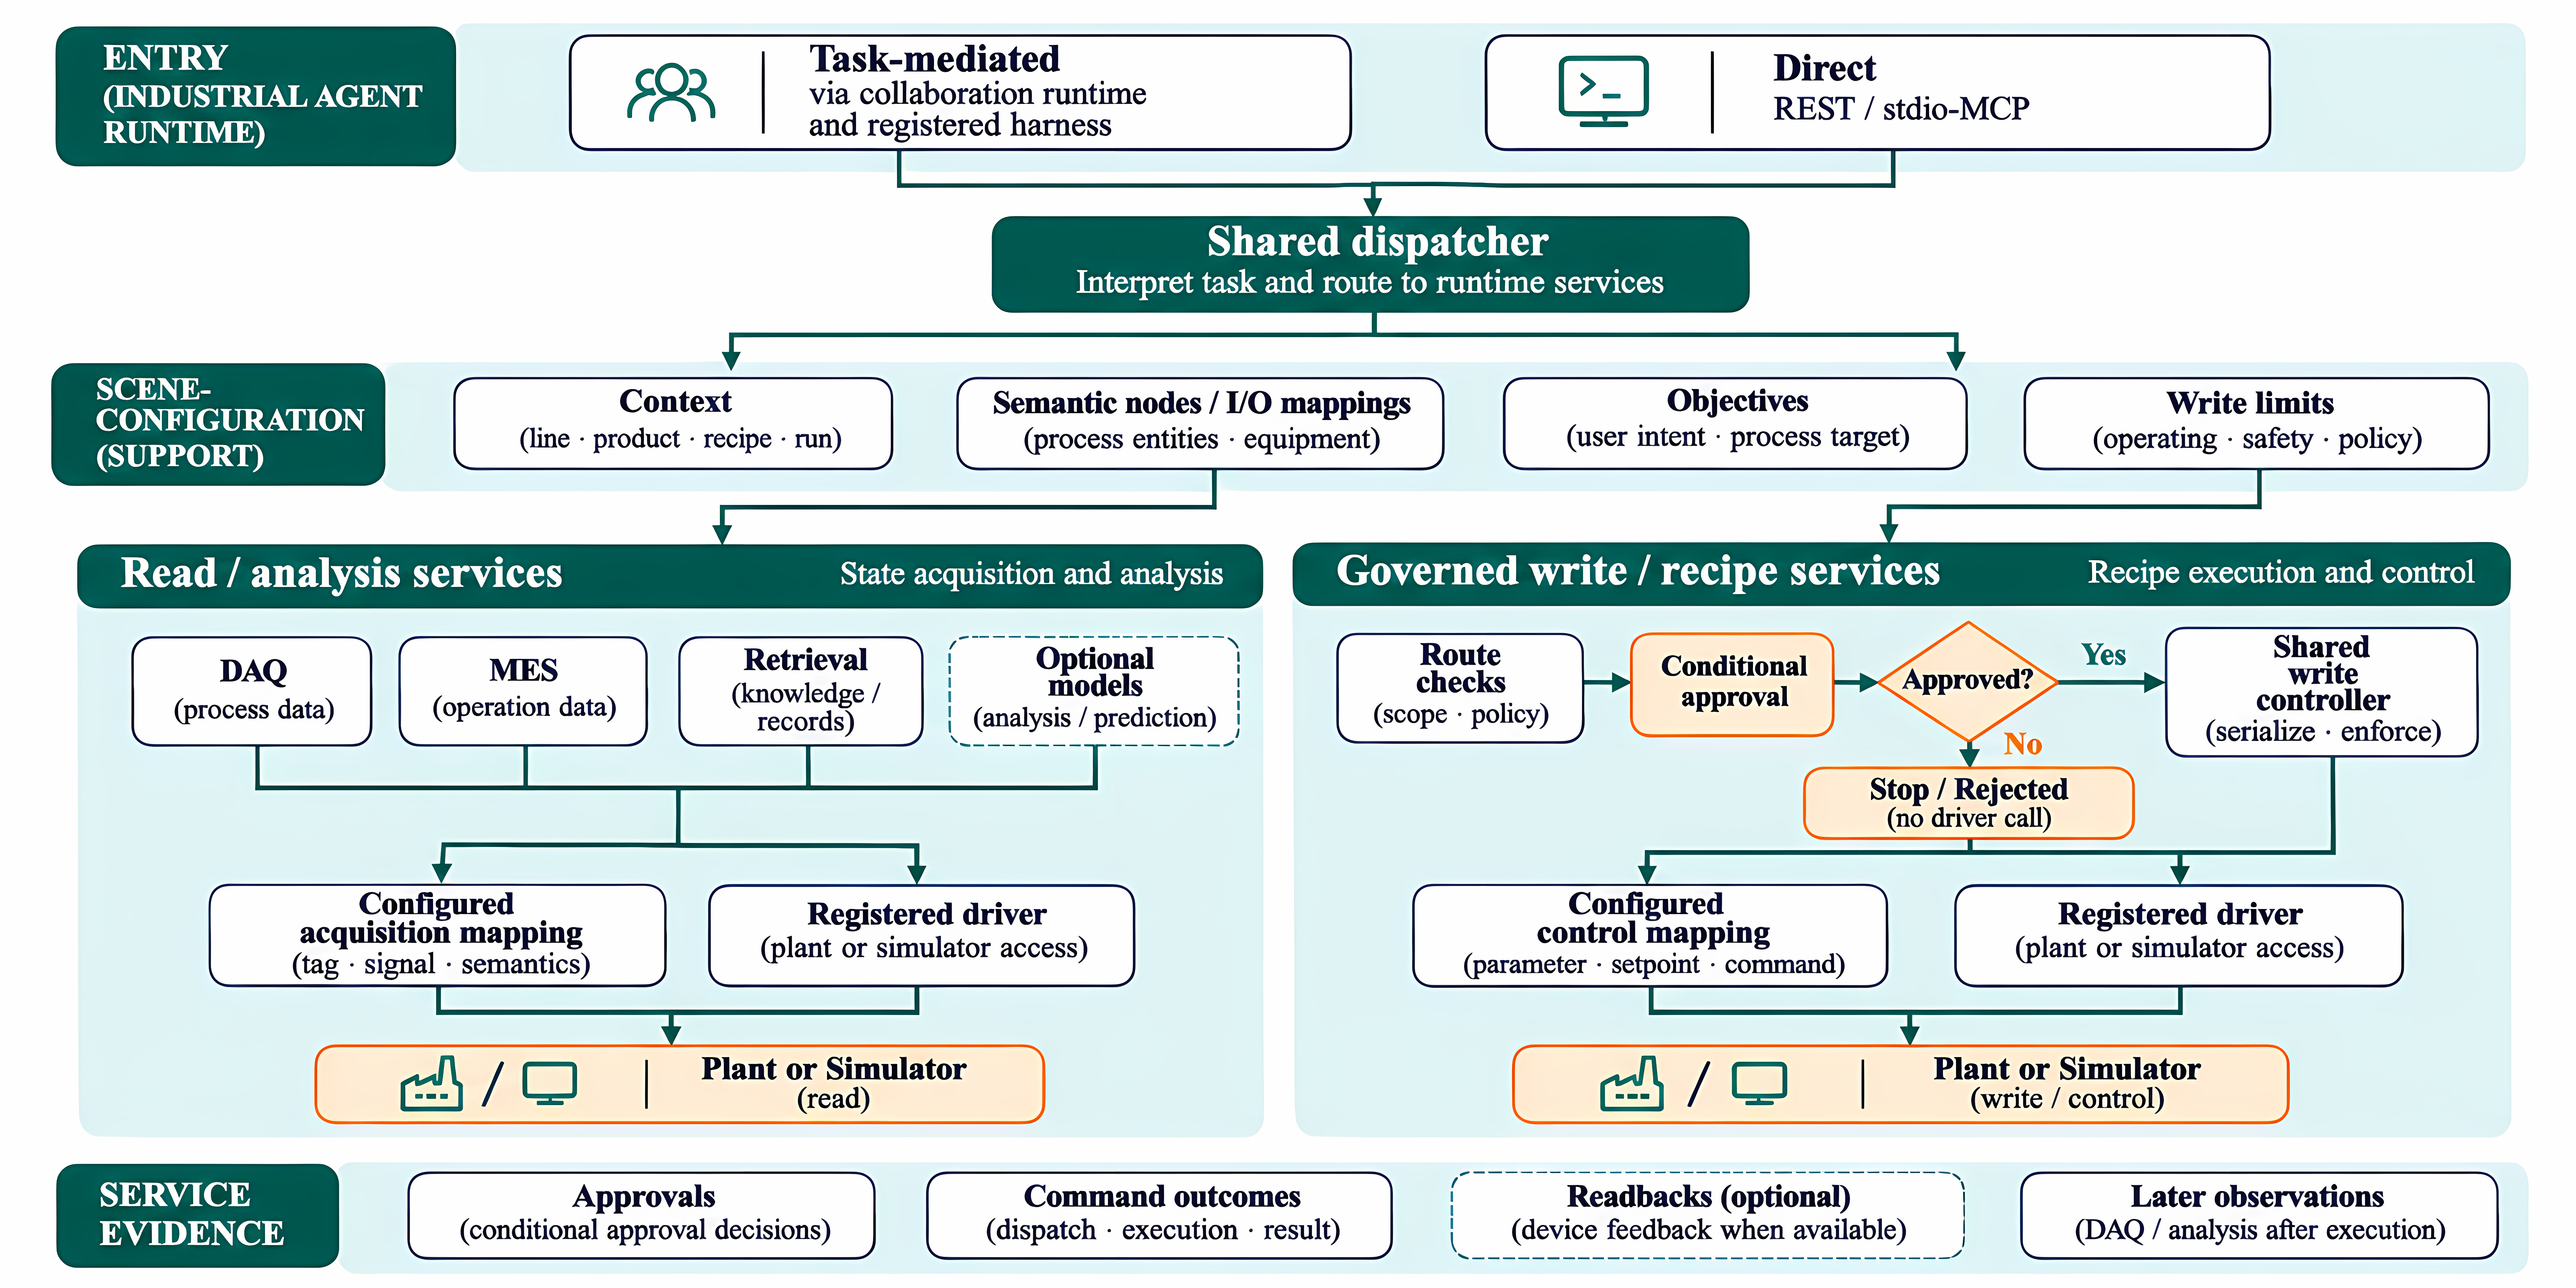
\includegraphics[width=\textwidth]{../figures/fig2.png}
\caption{Task-mediated and direct calls converge on the shared dispatcher, which routes requests to read/analysis or governed write/recipe services. The scene-configuration band supplies context, semantic I/O mappings, objectives, and write limits; it is configuration support rather than a third entry route. Read/analysis services connect DAQ, MES, retrieval, and optional models to acquisition mappings and registered drivers. The governed write path applies route checks and conditional approval before the shared write controller, then uses configured control mappings and drivers. The service-evidence band separates approvals, command outcomes, optional readbacks, and later observations. Evaluation uses simulator and mock-driver fixtures. The depicted limits are application checks and do not establish functional safety.}
\label{fig:arch}
\end{figure*}

\subsection{Design Rationale and Requirements}
\label{sec:principles}
The runtime must preserve process meaning across heterogeneous drivers,
provide a stable operation contract to registered harness adapters, and check
current authority and process limits before a write. It must also keep command
acceptance separate from later process observations. Scene configuration,
registered adapters, shared dispatch, route handlers, and service-owned
records implement these boundaries.

At task start, the context builder assembles the active production tuple and
relevant process summaries. This context informs a proposal but does not grant
write authority. When an operation is invoked, its handler resolves the live
state required by that route.

\subsection{Layered Architecture}
\label{sec:layers}
Task-mediated calls pass through the collaboration runtime, which coordinates
the task and invokes a registered harness adapter. The adapter presents the
agent's scoped tools and current task context; its binding and channel policy
constrain the available operations. Direct REST calls and the stdio-MCP
operation bridge skip task execution but converge on the same dispatcher. This
description applies to the operation bridge: MCP management and task methods
remain on their service routes.

Scene configuration has two consumers. The task route receives active context
and objectives, while operation services resolve node mappings and guards when
an operation executes. Read and analysis services group DAQ, MES data access,
retrieval, and optional models; write and recipe services handle control
operations. For a write mapping, the driver registry can select a configured
MES-REST adapter. At the field layer, input/output (I/O) mappings connect
semantic nodes to built-in or plugin drivers for a plant or simulator. Each
owning service retains its task, command, observation, or configuration
records and associates them with the actor and production context where
supported.

\subsection{Scene Configuration as the Integration Boundary}
\label{sec:scene-config}
Scene-specific process semantics are configured before an
agent task begins. The active line identifies the production context; product
and recipe records supply applicable targets and limits; the run record
provides the current operating state. Semantic nodes bind process variables
to direction-specific acquisition or control mappings, which the driver
registry resolves to supported protocol implementations. Here
\emph{semantic} denotes a named process variable with a direction, unit, and
configured mapping; it is not an OPC UA or Asset Administration Shell
information model. Each agent-facing operation is named and typed, so a harness does not need to
construct protocol-specific messages. A scene using an already registered
driver can supply different context and node mappings behind the same
operation contract. A protocol not present in the registry still requires a
driver adapter; configuration alone does not implement a new protocol.

In the cast-film simulator preset, for example, the MQTT command mapping
\texttt{linespeed-sp} controls line speed in m/min, while the distinct
\texttt{film-thickness} mapping supplies thickness in $\mu$m. A task can
refer to both nodes: a candidate is admitted against the control node's
limits, whereas a later DAQ observation describes thickness. Sharing MQTT does
not make either signal a substitute for the other.

Table~\ref{tab:scene-config} summarizes how the execution path uses the scene
description and distinguishes configuration-time bindings from checks against
live state. The context assembled for an agent turn is descriptive. Before a
write, the handler resolves the live state required by its route and applies
the current limits. Where a route supports context snapshots, approval is
bound to both the proposal and the context. The command receipt remains
separate from subsequent DAQ observations.

\begin{table*}[!t]
\centering
\caption{Scene configuration elements and their roles in the runtime path.}
\label{tab:scene-config}
\footnotesize
\setlength{\tabcolsep}{5pt}
\begin{tabularx}{\textwidth}{@{}>{\raggedright\arraybackslash}p{0.19\textwidth}>{\raggedright\arraybackslash}p{0.34\textwidth}X@{}}
\toprule
Element & Configured information & Runtime use\\
\midrule
Production context & Line, product, recipe, and run associations & Context construction for a task turn; route-dependent live-state checks before a write\\
Semantic I/O & Process variable, direction, unit, and node mapping & Acquisition uses the read mapping; accepted operations resolve the configured control mapping\\
Driver binding & Supported protocol driver and endpoint configuration & Driver registry selects the protocol implementation after operation checks\\
Operation admission & Engineering, baseline, product, and recipe limits; step and timing rules where configured & Route handler checks the candidate against current bounds and rejects inadmissible requests\\
Approval policy & Whether approval is required and the decision validity window & Pending request binds the proposed action; route-specific checks run after approval\\
Evidence ownership & Command receipt, verification grade, and later DAQ observations & Owning services retain command outcomes separately from process measurements\\
\bottomrule
\end{tabularx}
\end{table*}

\subsection{Cross-Module Execution Flow}
\label{sec:executionflow}
At the operation boundary, the shared dispatcher checks the predicates
declared for the named operation before selecting its handler. The handler
resolves live production state, applies route-specific guards and limits, and
requests any required approval before device I/O.

For an industrial operation $u$ by agent $a$ in channel $c$, define the
shared dispatch condition as
\begin{equation}
\mathcal{A}(a,c,u)=\bigwedge_{X\in\mathcal{C}(u)}X(a,c,u),
\label{eq:dispatch-contract}
\end{equation}
where $S$, $P$, $G$, and $B$ denote invocation scope, current channel policy,
applicable industrial grant, and the agent's binding to referenced resources,
respectively. $\mathcal{C}(u)\subseteq\{S,P,G,B\}$ is the set of predicates
declared for operation $u$; it always contains $S$ and $P$. The grant predicate
$G$ is included when the resolved channel, target line, and owner/grant policy
require it; explicit exemptions omit it. The binding predicate $B$ is included
when the operation declares resource references. An operation that declares
no references omits $B$. Each included check must pass before handler
selection. The policy predicate includes channel tool selection, profile, and duty-separation checks where
configured.

After these predicates pass, the selected route applies its operational
guards and any required approval. For example, an exploration request checks
the control binding and DAQ visibility before entering the governed write
path; an invisible target returns an error before a write. The checks performed
after approval depend on the route; Section~\ref{sec:modules} specifies the
single-node and recipe-operation paths.

For a direct REST call, the service establishes $a$ and $c$ before applying
these checks. An agent token must match the requested agent identifier; an
authenticated user must be the channel owner or an administrator. The manager
loads the channel-agent record and rechecks scope and policy, followed by any
applicable grant and binding checks. Handlers resolve live production state
from request identifiers and owning services.

Section~\ref{sec:modules} specifies route-level admission, timing, approval,
and evidence rules. A shared dispatcher alone does not establish that the two
entry paths behave identically.


